\chapter{Generating Exponential Random Variables}

\setcounter{problem}{1}
\section{Discussion}

\begin{fullwidth}

The goal of this lab is to generate random values from the exponential distribution using the {\em inverse transform method}.  You will show the histogram of the random values and then show the theoretical exponential distribution on top to verify your results. You will reuse your exponential distribution random variable generator for the central limit theorem lab later. Use filename {\tt stats/plot\_rexp.py} for the plotting code, but you will stick your exponential functions into the usual {\tt stats/stats.py} file.

\section{Steps}

\step First, create a function called {\tt rexp(lambduh)} in {\tt stats/stats.py} that returns a random value from the exponential distribution using the inverse transform method. To do that, you need the inverse {\em cumulative distribution function} (CDF) for the exponential distribution $Exp(\lambda)$. The {\em probability density function} for the exponential distribution is:

\[
p = F(x; \lambda) = \lambda e^{-\lambda x}
\]

\noindent Therefore the inverse function to get the $x$ value associated with a probability $p$, we use

\[
x = F^{-1}(p; \lambda) = -\frac{ln(1-p)}{\lambda}
\]

\noindent Your function should look like the following:

\begin{pyverbatim}
def rexp(lambduh): # lambduh mispelled to avoid clash with lambda in python
    # u = get value from U(0,1) then
    # return F^-1(u) for exp cdf F^-1
\end{pyverbatim}

\noindent Use your {\tt runif01()} function from previous labs.

\step To plot things, create file {\tt stats/plot\_rexp.py} and get a sample of exponential random variables into variable {\tt X} of size N from $Exp(1.5)$ using your {\tt rexp()}. I usually define constants to make the code more readable:

\begin{pyverbatim}
N = 1000
LAMBDUH = 1.5
\end{pyverbatim}

\noindent then I can call {\tt rexp(LAMBDUH)} and change LAMBDUH everywhere in my code by just changing the constant. In this case, there's no real need but it's good practice.

\step  Plot a histogram of you are sample with {\tt bins=40, normed=1}.  You should see something like this:

\scalebox{.4}{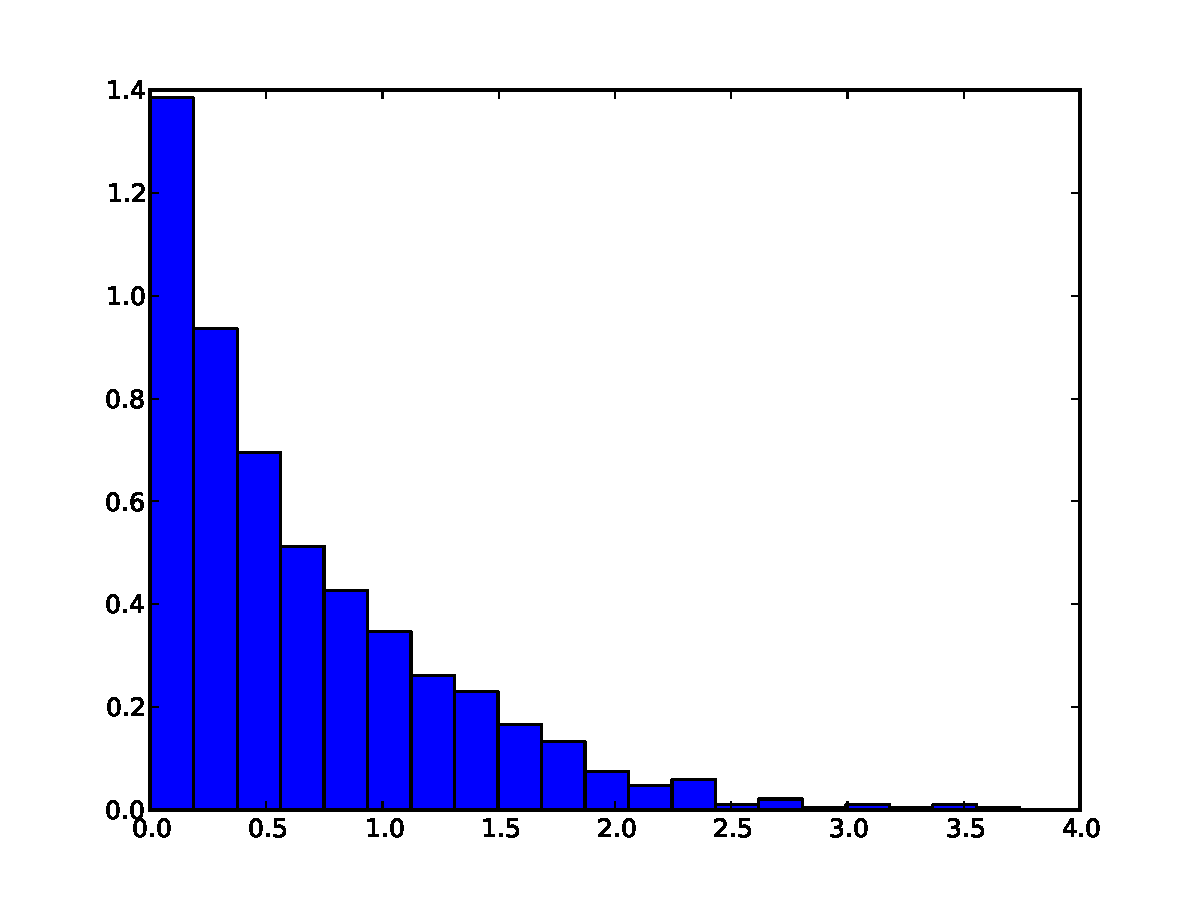
\includegraphics{figures/exp-1_5-density.pdf}}

\noindent {\bf How do we know that this accurately represents the exponential distribution? We plot the theoretical distribution on top with a red line.}\\

\step Since it's easy, let's define our own exponential probability density function in {\tt stats/stats.py} as follows:

\begin{pyverbatim}
def exppdf(x, lambduh):
    ...
\end{pyverbatim}

\noindent When you call it, make sure use the same lambduh.

\step Now, before the call to function {\tt show()}, plot the theoretical distribution so that we can see both at once:

\scalebox{.4}{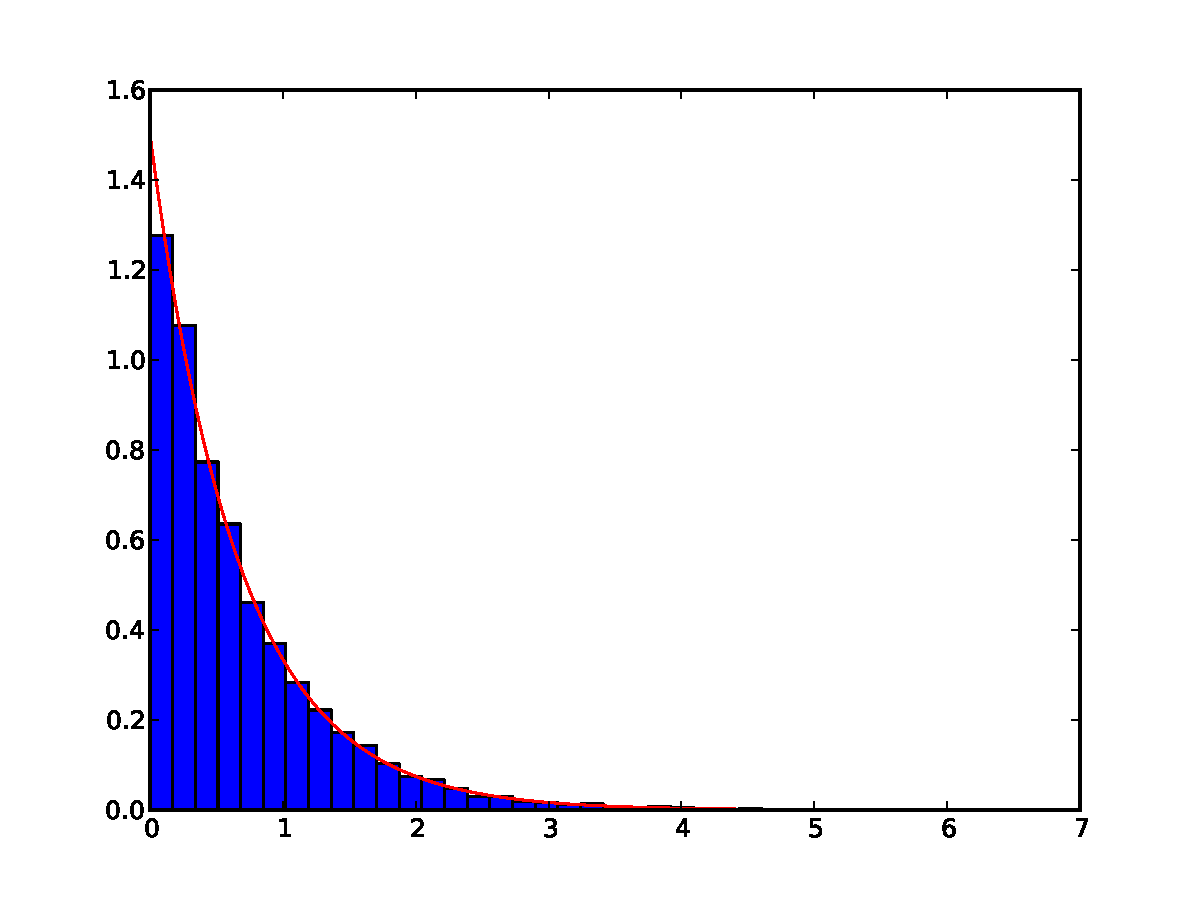
\includegraphics{figures/exp-1_5-density-fancy.pdf}}


\begin{callout}{\bcplume}
{\bf Deliverables}. Make sure that {\tt stats/stats.py} has the new functions and that {\tt stats/plot\_rexpr.py} is correctly committed to your repository and pushed to github. 
\end{callout}

\end{fullwidth}
